\definecolor{zzttqq}{rgb}{0.15,0.35,0.15}

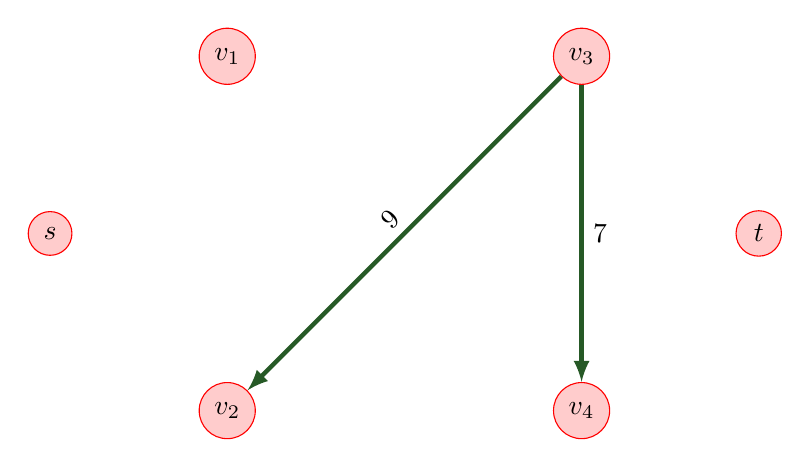
\begin{tikzpicture}[x=1.5cm, y=1.5cm]
	%\fill (-3.2,0) circle (0.1pt)node[anchor=east] {$20$};
	%\fill (3.2,0) circle (0.1pt)node[anchor=west] {$-20$};
    \node[circle,draw=red,fill=red!20!] (v1) at (-1.5,1.5) {$v_1$};
    \node[circle,draw=red,fill=red!20!] (v3) at (1.5,1.5) {$v_3$};
    \node[circle,draw=red,fill=red!20!] (t) at (3,0) {$t$};
    \node[circle,draw=red,fill=red!20!] (v4) at (1.5,-1.5) {$v_4$};
    \node[circle,draw=red,fill=red!20!] (v2) at (-1.5,-1.5) {$v_2$};
    \node[circle,draw=red,fill=red!20] (s) at (-3,0) {$s$};
    \DoubleLine{s}{v1}{latex-, color=zzttqq, ultra thick}{7}{-latex, color=zzttqq, ultra thick}{9}
    \DoubleLine{s}{v2}{latex-, color=zzttqq, ultra thick}{11}{-latex, color=zzttqq, ultra thick}{2}
    \DoubleLine{v2}{v1}{latex-, color=zzttqq, ultra thick}{1}{-latex, color=zzttqq, ultra thick}{3}
    \DoubleLine{v1}{v3}{latex-, color=zzttqq, ultra thick}{8}{-latex, color=zzttqq, ultra thick}{4}
    \DoubleLine{v2}{v4}{latex-, color=zzttqq, ultra thick}{10}{-latex, color=zzttqq, ultra thick}{4}
	%\draw[-latex, color=zzttqq, ultra thick]  (v2) edge node[above,color=black]{10/14} (v4);
	\draw[-latex, color=zzttqq, ultra thick]  (v3) edge node[rotate=45,above,color=black]{9} (v2);
	\draw[-latex, color=zzttqq, ultra thick]  (v3) edge node[right,color=black]{7} (v4);
    \DoubleLine{v3}{t}{latex-, color=zzttqq, ultra thick}{15}{-latex, color=zzttqq, ultra thick}{5}
	\DoubleLine{v4}{t}{latex-, color=zzttqq, ultra thick}{3}{-latex, color=zzttqq, ultra thick}{1}
\end{tikzpicture}